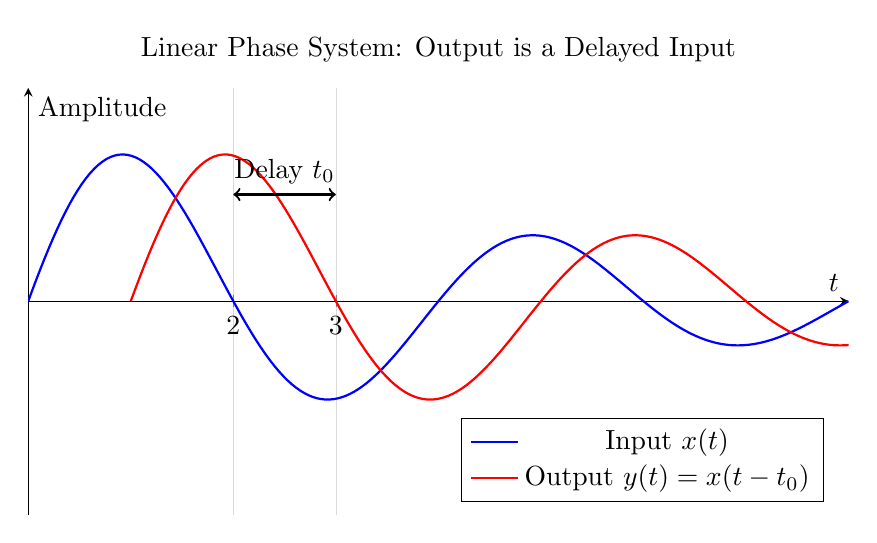
\begin{tikzpicture}
	\begin{axis}[
		width=12cm,
		height=7cm,
		title={Linear Phase System: Output is a Delayed Input},
		xlabel={$t$},
		ylabel={Amplitude},
		axis lines=middle,
		xmin=0, xmax=8,
		ymin=-1.2, ymax=1.2,
		xtick={2,3},
		ytick=\empty,
		grid=major,
		grid style={line width=.1pt, draw=gray!30},
		legend pos=south east,
		no marks,
		]
		\addplot[blue, thick, domain=0:8, samples=200] {sin(deg(2*pi*x/4)) * exp(-0.2*x)};
		\addlegendentry{Input $x(t)$};
		
		\addplot[red, thick, domain=1:8, samples=200] {sin(deg(2*pi*(x-1)/4)) * exp(-0.2*(x-1))};
		\addlegendentry{Output $y(t) = x(t-t_0)$};
		
		\draw[<->, thick] (axis cs:2,0.6) -- (axis cs:3,0.6) node[midway, above] {Delay $t_0$};
	\end{axis}
\end{tikzpicture}










